% Versión de lectura en español de main.tex. La versión para la revista es
% main.tex (inglés); este archivo no se envía. Si cambia main.tex, hay que
% actualizar esta traducción a mano.
\documentclass[preprint,11pt]{elsarticle}

\usepackage[spanish,es-noshorthands,es-tabla]{babel}
\usepackage{amsmath}
\usepackage{booktabs}
\usepackage{graphicx}
\usepackage{xcolor}
\usepackage{tikz}
\usetikzlibrary{positioning,arrows.meta,fit,backgrounds}
\usepackage[hidelinks]{hyperref}
\usepackage{url}

\newcommand{\todo}[1]{\textcolor{red}{[PENDIENTE: #1]}}

\journal{Computers in Industry}
\abstracttitle{Resumen}
\myfooter[L]{Versión de lectura en español. El manuscrito que se envía a \emph{Computers in Industry} es la versión en inglés.}
\makeatletter\def\@elsarticlehighlightstitle{Aspectos destacados}\makeatother

\begin{document}

\begin{frontmatter}

\title{De la detección a la acción: cerrando el bucle autonómico de una línea de fabricación autocoordinada con planificadores basados en reglas y en LLM con recuperación aumentada}

\author[a,b]{Manuel S\'anchez\corref{cor1}}
\ead{mbsanchez@unet.edu.ve}
\author[b]{Ernesto Exposito}
\ead{ernesto.exposito@univ-pau.fr}
\cortext[cor1]{Autor de correspondencia.}
\address[a]{Universidad Nacional Experimental del T\'achira, San Crist\'obal, Venezuela}
\address[b]{Univ Pau \& Pays Adour / E2S UPPA, Laboratoire d'informatique de l'Universit\'e de Pau et des Pays de l'Adour (LIUPPA), EA3000, 64000 Pau, Francia}

\begin{abstract}
Las arquitecturas autonómicas para la Industria~4.0 prometen una producción que se autoconfigura, se autorrepara y se autooptimiza, pero los sistemas publicados a menudo se quedan en la detección. Revisamos nuestra propia arquitectura de fabricación autocoordinada de 2020 y su simulador, y comprobamos que implementa las fases Monitor y Analyze, pero no Plan, Execute ni una base de conocimiento: las condiciones detectadas solo producen un mensaje en un registro. Portamos el simulador a un motor sin interfaz gráfica y con pruebas, sobre el conjunto de datos de la línea de producción de Bosch, y cerramos el bucle con un espacio de acciones construido sobre las estaciones gemelas paralelas de la línea, un validador simbólico, inyección de fallos (escalón, intermitentes y deriva) y un modelo de efectos explícito. Comparamos planificadores basados en reglas con planificadores basados en modelos de lenguaje de gran tamaño (LLM), con y sin conocimiento operativo recuperado, sobre un modelo local de 7B (Qwen2.5) y un modelo de frontera (Claude Fable~5.1), usando una traza de desarrollo para el diseño y tres trazas reservadas para la evaluación. Cerrar el bucle de forma ingenua es perjudicial: conectar las alarmas originales directamente a acciones es peor que no hacer nada. El cuello de botella es el triaje de alarmas, no la planificación. Un test clásico de detección adaptativa de cambios recupera entre el 52 y el 54\,\% del retraso causado por los fallos. Con el modelo de 7B, el planificador con recuperación aumentada recupera el 20\,\%; con el modelo de frontera, el mismo diseño recupera el 58\,\% y supera a la mejor regla en 50 de 72 escenarios ($p=0{,}003$), con una ganancia agregada que no es significativa en conjunto pero sí grande en los fallos intermitentes, que derrotan a todas las reglas. Usado en cambio como veto sobre el detector original, el modelo de frontera sobreinterpreta un artefacto de cómo ese detector agrupa las alarmas. La capacidad del modelo importa, pero no puede reparar una interfaz Analyze--Knowledge mal diseñada.
\end{abstract}

\begin{highlights}
\item La arquitectura autonómica de 2020 solo implementaba detección, sin planificación ni ejecución.
\item Conectar las alarmas heredadas directamente a reparaciones es peor que no hacer nada.
\item Un test clásico de detección adaptativa de cambios es un baseline sólido para el triaje.
\item Un LLM de frontera con conocimiento recuperado lo iguala y gana en fallos intermitentes.
\item Como veto sobre alarmas agrupadas, el LLM de frontera es engañado por un artefacto del detector.
\end{highlights}

\begin{keyword}
Computación autonómica \sep MAPE-K \sep Industria 4.0 \sep Modelos de lenguaje de gran tamaño \sep Generación aumentada por recuperación \sep Gestión de fallos
\end{keyword}

\end{frontmatter}

% =====================================================================
\section{Introducción}
\label{sec:intro}

La computación autonómica propone sistemas que se gestionan a sí mismos mediante un bucle Monitor--Analyze--Plan--Execute sobre una base de conocimiento compartida (MAPE-K)~\cite{kephart2003vision,weyns2020introduction}. En la fabricación este bucle resulta atractivo porque las líneas de producción se degradan continuamente y la supervisión humana no escala: una línea que se autorrepara detectaría una estación que se degrada y se reconfiguraría antes de que el retraso se acumule.

En 2020 propusimos una arquitectura para procesos de fabricación autocoordinados con propiedades self-* y la evaluamos con un simulador, SSACSimulator, sobre el conjunto de datos de la línea de producción de Bosch~\cite{sanchez2020selfstar,sanchez2020jii}. Al revisar ese código seis años después, comprobamos que solo implementa las fases Monitor y Analyze. Cuando uno de sus tres detectores se dispara, el simulador escribe \emph{``launching the autonomous cycle for reconfiguration''} en un panel de registro; no se produce ningún plan y no se ejecuta nada. El bucle se anunciaba, pero no se cerraba.

Este artículo lo cierra y se pregunta qué hace falta realmente para cerrarlo. Dos desarrollos hacen oportuna la pregunta. Primero, los modelos de lenguaje de gran tamaño (LLM) se proponen cada vez más como planificadores para la toma de decisiones industriales, desde el control de sistemas de producción modulares~\cite{xia2023towards} hasta la planificación y programación avanzadas~\cite{li2026a4ps}. Segundo, la generación aumentada por recuperación (RAG)~\cite{lewis2020rag} es una candidata natural para el componente Knowledge de MAPE-K: en lugar de una ontología construida a mano, el planificador recupera el historial operativo que necesita. Si alguno de los dos ayuda, y frente a qué baseline, es una cuestión empírica.

Nuestras contribuciones son:
\begin{enumerate}
  \item Un port fiel, sin interfaz gráfica y con pruebas del simulador de 2020, y un análisis de su capa Analyze sobre los datos publicados: uno de los tres detectores es inalcanzable, otro se ejercita con el 0{,}004\,\% de los eventos y el tercero se dispara de forma rutinaria en una traza sin fallos (sección~\ref{sec:revisit}).
  \item Las fases Plan y Execute que faltaban: un espacio de acciones basado en las estaciones ``gemelas'' paralelas de la línea de Bosch, un validador simbólico, inyección de fallos con tres formas y un modelo de efectos explícito y parametrizado cuyos supuestos no verificables se barren en lugar de fijarse (sección~\ref{sec:loop}).
  \item Una comparación de planificadores basados en reglas con planificadores LLM con y sin conocimiento recuperado, y con un híbrido en el que un test estadístico hace el triaje y el LLM veta, sobre un modelo local de 7B y un modelo de frontera, con un protocolo que separa una traza de desarrollo de tres trazas reservadas (secciones~\ref{sec:planners}--\ref{sec:results}).
  \item Evidencia de que el cuello de botella para cerrar el bucle es el triaje de alarmas y no la planificación; de que la capacidad del LLM es decisiva para el triaje con recuperación aumentada; y de que un modelo capaz puede ser engañado por un artefacto del detector del que recibe las alarmas (sección~\ref{sec:discussion}).
\end{enumerate}

Todo el código, los scripts de procesamiento de datos, los prompts, las respuestas almacenadas de los modelos y los resultados están disponibles (sección~\ref{sec:availability}).

% =====================================================================
\section{Antecedentes y trabajo relacionado}
\label{sec:related}

\paragraph{Computación autonómica y sistemas autoadaptativos}
El modelo de referencia MAPE-K~\cite{kephart2003vision} estructura un sistema autogestionado como un bucle de realimentación en torno a un recurso gestionado. La ingeniería de esos bucles es el objeto de la literatura sobre sistemas autoadaptativos~\cite{weyns2020introduction}, que subraya que la fase Analyze debe separar el cambio real del ruido antes de planificar cualquier adaptación. Recientemente se han estudiado los LLM como componentes de esos bucles: una revisión del estado del arte y hoja de ruta organiza sus usos potenciales en torno a las funciones de MAPE-K~\cite{li2024genai,li2024exploring}; se han integrado agentes basados en LLM en sistemas multiagente basados en MAPE-K~\cite{nascimento2023selfadaptive}; y MAPER extiende MAPE-K con un componente de razonamiento basado en LLM para manejar situaciones imprevistas en tiempo de ejecución~\cite{alves2026maper}. Nuestro estudio se diferencia en que sitúa un LLM dentro del bucle de un sistema industrial cuyo detector heredamos sin cambios, y en que lo mide frente a baselines fuertes sin LLM sobre datos reservados.

\paragraph{Propiedades self-* en la fabricación}
Nuestro trabajo previo integró sistemas multiagente, orientación a servicios y computación autonómica para la coordinación de procesos en la Industria~4.0~\cite{sanchez2020selfstar,sanchez2020jii,sanchez2020survey}. El presente artículo reexamina empíricamente esa arquitectura en lugar de proponer una nueva.

\paragraph{Detección de cambios}
Detectar un cambio en la tasa de un flujo de eventos es un problema clásico~\cite{basseville1993detection}. Nuestros baselines basados en reglas más fuertes son instancias sencillas: un test de Poisson frente a una tasa base estática y un test frente al historial reciente del mismo flujo.

\paragraph{LLM y recuperación en la toma de decisiones industriales}
RAG condiciona un modelo de lenguaje con documentos recuperados para cada consulta~\cite{lewis2020rag}. En la fabricación, se han combinado agentes LLM con gemelos digitales para planificar y controlar la producción modular~\cite{xia2023towards} y se han aplicado a la planificación y programación avanzadas~\cite{li2026a4ps}, y una revisión reciente de los LLM para el diagnóstico de fallos en la fabricación inteligente cubre, entre otras funciones, la fusión de conocimiento industrial con recuperación aumentada~\cite{thuan2026review}. Nuestro diseño incluye deliberadamente un baseline estadístico fuerte y reglas de control que aíslan lo que el LLM aporta más allá de ellos.

% =====================================================================
\section{El sistema de 2020, revisado}
\label{sec:revisit}

\subsection{Simulador y datos}
SSACSimulator es un simulador de eventos discretos en Qt/C++. Un modelo de proceso, derivado del conjunto de datos Bosch Production Line Performance~\cite{bosch2016kaggle}, describe 52 estaciones en cuatro sublíneas más los nodos de inicio y fin, 285 transiciones (84 de ellas flujos principales), un tiempo de ciclo de 6\,420~min y 1\,183\,165 casos. Cuatro trazas de eventos de 100\,000 transiciones cada una reproducen movimientos de piezas registrados; abarcan entre 54 y 168 horas de producción.

\subsection{Port sin interfaz gráfica}
Portamos a Python el núcleo de simulación (unas 1\,440 líneas de lógica en C++; las $\sim$960 restantes son interfaz gráfica). El port reproduce el comportamiento del original tal como se lee en su código fuente, incluidos detalles que cambian los resultados: umbrales calculados en precisión simple, un límite de carga de 100\,000 eventos y una regla permisiva para las filas mal formadas. Un camino rápido avanza solo las piezas que pueden salir del sistema; el bucle original por tick se conserva como oráculo de pruebas, y una prueba de regresión comprueba que ambos producen detecciones, decisiones y tiempos de vida de pieza idénticos. Una ejecución tarda entre 0{,}2 y 0{,}4~s. La batería de pruebas tiene 87 tests.

\subsection{Lo que hace realmente la capa Analyze}
El original implementa tres detectores: una estación cuyo tiempo medio de transición supera 1{,}3 veces su referencia; más del 10\,\% de las estaciones marcadas dentro de un mismo lote de eventos simultáneos; y un tiempo de vida medio de las piezas que supera 1{,}1 veces el tiempo de ciclo. En la primera traza solo se dispara el segundo (39 alarmas). El detector de fallos predichos depende de una etiqueta de un clasificador que es positiva en 15 de 400\,000 eventos en el conjunto de las trazas (0{,}004\,\%). El detector global es inalcanzable: el tiempo de vida medio de las piezas (636~min) está un orden de magnitud por debajo de su umbral (7\,062~min). Por último, 45 de las 285 transiciones tienen un tiempo de referencia cero, de modo que cualquier duración positiva marca su estación.

Plan, Execute y Knowledge están ausentes. Ese es el punto de partida del resto del artículo.

% =====================================================================
\section{Cerrar el bucle}
\label{sec:loop}

La figura~\ref{fig:loop} resume el bucle cerrado. Los componentes añadidos en este trabajo aparecen sombreados.

\begin{figure}[t]
\centering
\resizebox{\linewidth}{!}{%
\begin{tikzpicture}[
  node distance=7mm and 13mm,
  box/.style={draw, rounded corners=2pt, minimum width=24mm, minimum height=8mm, align=center, font=\small},
  new/.style={box, fill=black!8},
  >={Stealth[length=2mm]}]
  \node[box] (mon) {Monitor\\[-1pt]\scriptsize reproducción de eventos};
  \node[box, right=of mon] (ana) {Analyze\\[-1pt]\scriptsize detectores heredados};
  \node[new, right=of ana] (plan) {Plan\\[-1pt]\scriptsize reglas / LLM};
  \node[new, right=of plan] (exe) {Execute\\[-1pt]\scriptsize modelo de efectos};
  \node[new, below=of ana] (k) {Knowledge\\[-1pt]\scriptsize memoria + tasas base};
  \node[new, below=of plan] (val) {Validador simbólico\\[-1pt]\scriptsize grafo del proceso};
  \node[box, above=of plan, minimum width=95mm] (line) {Línea de producción (trazas de Bosch) + fallos inyectados};
  \draw[->] (mon) -- (ana);
  \draw[->] (ana) -- node[above, font=\scriptsize]{alarmas} (plan);
  \draw[->] (plan) -- node[right, font=\scriptsize]{acciones} (val);
  \draw[->] (val.east) -| (exe.south);
  \draw[->] (exe.north) -- (exe.north |- line.south);
  \draw[->] (line.west) -| (mon.north);
  \draw[<->] (k) -- (plan);
  \draw[->] (ana) -- (k);
\end{tikzpicture}}
\caption{El bucle MAPE-K cerrado. Blanco: presente en el sistema de 2020. Gris: añadido en este trabajo.}
\label{fig:loop}
\end{figure}

\subsection{Estaciones gemelas y espacio de acciones}
La línea de Bosch está formada por pares de estaciones paralelas (y algunos tríos) que comparten predecesoras y sucesoras y se reparten la carga casi por igual; por ejemplo, las estaciones L0\_S2 y L0\_S3 procesan 339\,345 y 334\,054 casos. Identificamos las gemelas automáticamente a partir del solapamiento de sus conjuntos de predecesoras y sucesoras en los flujos principales: 29 de las 52 estaciones tienen una. Desviar una pieza de una estación a su gemela mantiene coherente su trayectoria, lo que hace del desvío una acción con sentido físico. El espacio de acciones es \textsc{Reroute}(S, T, $f$), que desvía una fracción $f$ de las piezas que entran en S hacia su gemela T; \textsc{Restore}(S); \textsc{Maintenance}(S, $d$), que repara S durante $d$ minutos; y \textsc{NoOp}.

\subsection{Validador simbólico}
Toda acción, de cualquier planificador, se comprueba contra el grafo del proceso y las intervenciones en curso antes de ejecutarse: las estaciones deben existir, el destino de un desvío debe ser una gemela estructural, los desvíos no deben formar cadenas y una estación no puede repararse dos veces a la vez. El validador nunca juzga si una acción es buena idea, solo si es admisible.

\subsection{Modelo de efectos}
La simulación está guiada por la traza: los instantes de inicio proceden de los datos registrados y no se desplazan; los fallos y las acciones actúan sobre las duraciones de las transiciones, y el tiempo de vida de una pieza es la suma de las duraciones de sus transiciones. Por tanto, el retraso no se propaga en forma de colas; el modelo estima el tiempo perdido por pieza. Una ``transición'' de Bosch es el tiempo entre dos marcas de estación y mide sobre todo espera: su mediana es 0~min y su percentil 90 es 30~min, pero su percentil 99 llega a 4\,000--6\,000~min. Por ello los efectos son \emph{aditivos} y proporcionales al tiempo de proceso de cada estación $\tau_S$ (la mediana de sus transiciones de hasta 60~min), nunca multiplicativos sobre una transición que incluye días de almacenamiento. $\tau_S$ vale entre 6 y 12~min y es muy estable entre trazas. El modelo de efectos es:
\begin{itemize}
  \item \textbf{Fallo} de factor $k$ en S: $+(k(t)-1)\,\tau_S$ en cada transición que sale de S, donde $k(t)$ es un \emph{escalón} ($k$ desde $t_0$), \emph{intermitente} ($k$ durante 60~min, 1 durante 120~min, y así sucesivamente) o una \emph{deriva} (crece linealmente de 1 a $k$ en 600~min).
  \item \textbf{Desvío}: una fracción determinista de las piezas (seleccionadas mediante un hash del identificador del caso) va a T, que añade entonces $\alpha\,f\,\tau_T$ por la carga extra.
  \item \textbf{Mantenimiento}: los fallos de S que empezaron antes del final de la reparación se eliminan al terminar esta. Durante la reparación, en modo \emph{contingencia} (por defecto) una capacidad de respaldo fuera del modelo procesa las piezas, añadiendo $0{,}5\,\tau_S$; en modo \emph{parada} las piezas esperan a que termine la reparación. Reparar una estación sana cuesta y no arregla nada, y eso es lo que encarece las falsas alarmas.
\end{itemize}
El conjunto de datos está anonimizado y no proporciona capacidades, tiempos de reparación ni fallos etiquetados, de modo que todos los fallos son sintéticos y todo parámetro que no pudimos fundamentar en los datos (severidad $k$, tiempo de reparación $d$, congestión $\alpha$, modo de mantenimiento) se varía en un análisis de sensibilidad (sección~\ref{sec:sweep}).

% =====================================================================
\section{Planificadores}
\label{sec:planners}

Todos los planificadores reciben, para cada alarma, la alarma y el estado de sus propias intervenciones anteriores. Ninguno ve los fallos inyectados. Todos responden del mismo modo ante una estación que consideran averiada: desviar a una gemela libre si existe y, después, reparar.

\subsection{Planificadores basados en reglas}
\begin{itemize}
  \item \textbf{Ingenuo}: actúa sobre toda estación nombrada en una alarma.
  \item \textbf{Calibrado}: actúa cuando el número de alarmas de una estación en 120~min es improbable (cola de Poisson, $\alpha=10^{-3}$) bajo su tasa base, aprendida en una traza sin fallos \emph{distinta}.
  \item \textbf{Adaptativo}: el mismo test, frente a la tasa observada en las 24~h anteriores de la misma traza, de forma causal, tras un calentamiento de 8~h.
  \item \textbf{Adaptativo + veto por carga} (control): la regla adaptativa, ignorando las estaciones que reciben carga que el propio controlador desvió hacia ellas.
  \item \textbf{Solo gemelas} (control): actúa sobre toda estación marcada que tenga una gemela libre e ignora las demás.
\end{itemize}
Los dos controles no son métodos propuestos; implementan como reglas simples comportamientos observados en planificadores LLM, de modo que la contribución de un LLM se mide más allá de ellos.

\subsection{Planificadores LLM}
Para cada alarma con estaciones accionables, el LLM debe devolver, para cada una de ellas, un veredicto (\emph{degradada}, \emph{normal}, \emph{autoinducida} o \emph{evidencia insuficiente}) seguido de un tipo de acción (ninguna, reparar, o desviar y reparar). La salida está restringida por un esquema JSON cuyos nombres de estación se limitan a las accionables, de modo que el decodificador no puede inventar una estación. El código elige la gemela, descarta toda acción incoherente con el propio veredicto del modelo y pasa el resto al validador.
\begin{itemize}
  \item \textbf{C1} recibe la alarma, las estaciones accionables, si cada una tiene una gemela libre y las intervenciones en curso: la misma información estructural que las reglas.
  \item \textbf{C2 (RAG)} recibe además conocimiento recuperado de la memoria operativa del controlador: para cada estación, las alarmas observadas en las últimas 2 y 24~h frente al número que predice su tasa base sin fallos, si el controlador le está desviando carga, si sus alarmas bajaron tras reparaciones anteriores y sus registros más recientes. La recuperación se indexa por estación y se ordena por recencia; todas las estadísticas las calcula el código.
  \item \textbf{Híbrido}: el test adaptativo de detección de cambios selecciona las estaciones; el LLM, con el conocimiento de C2, confirma o veta y elige la acción. Una estación vetada no se vuelve a examinar durante 120~min.
\end{itemize}

\paragraph{Modelos}
Usamos Qwen2.5-7B-Instruct~\cite{qwen2024}, cuantizado a 4 bits y servido localmente con Ollama~\cite{ollama} a temperatura~0; y Claude Fable~5.1 (Anthropic), accedido mediante el Claude Agent SDK~\cite{anthropic2026agentsdk} con el esfuerzo en \emph{low}, sin herramientas y sin fuentes de contexto externas. El modelo de frontera no expone un ajuste de temperatura, por lo que sus ejecuciones no son reproducibles bit a bit; todas las respuestas de ambos modelos se almacenan, lo que hace que todos los experimentos puedan volver a reproducirse.

% =====================================================================
\section{Protocolo experimental}
\label{sec:protocol}

\paragraph{Escenarios}
Se inyecta un fallo de factor $k=3$ 600~min después del inicio de una traza en una de ocho estaciones, cuatro con gemela (L0\_S2, L0\_S4, L0\_S6, L3\_S35) y cuatro sin ella (L0\_S1, L0\_S8, L3\_S29, L3\_S33), todas con tiempos de proceso observables en cada traza, con una de las tres formas de fallo. Cada traza tiene además una ejecución sin fallos. Las reparaciones duran 60~min, $\alpha=0{,}5$, y el mantenimiento funciona en modo contingencia salvo que se indique lo contrario.

\paragraph{Trazas de desarrollo y reservadas}
Los prompts y el contexto recuperado se diseñaron y revisaron solo sobre la primera traza, con cuatro casos de desarrollo; cada versión y sus resultados quedaron registrados. Las otras tres trazas están reservadas: sobre ellas los prompts se ejecutaron una vez, congelados. Las reglas calibradas aprenden siempre sus tasas base en una traza distinta de aquella en la que se evalúan.

\paragraph{Métricas}
Cada ejecución reproduce la misma traza, de modo que cada pieza se compara consigo misma en una ejecución de referencia sin fallos. El \emph{retraso en exceso} de una ejecución es la suma, sobre las piezas, de su tiempo de vida adicional. La \emph{recuperación agregada} de un planificador sobre un conjunto de escenarios es $1-\sum \text{exceso(planificador)} / \sum \text{exceso(no hacer nada)}$: 1 elimina el coste de los fallos; 0 no es mejor que no hacer nada; los valores negativos significan que las propias acciones del planificador cuestan más que los fallos. El \emph{coste de las falsas alarmas} es el retraso en exceso por hora en las ejecuciones sin fallos. Un \emph{acierto específico} cuenta una acción sobre la estación averiada solo si el mismo planificador, en la misma traza sin el fallo, no actuó sobre esa estación en un margen de $\pm$120~min; excluye las reparaciones de rutina que coinciden por casualidad con el fallo.

\paragraph{Estadística}
Los planificadores se comparan sobre escenarios pareados con la prueba de rangos con signo de Wilcoxon sobre el retraso en exceso~\cite{wilcoxon1945}, con ajuste de Holm~\cite{holm1979}, y con intervalos bootstrap al 95\,\%~\cite{efron1993bootstrap} para la diferencia de recuperación agregada, remuestreando los escenarios dentro de su traza (10\,000 remuestreos).

% =====================================================================
\section{Resultados}
\label{sec:results}

\subsection{Planificadores basados en reglas y sensibilidad}
\label{sec:sweep}
La tabla~\ref{tab:sweep} recoge los planificadores basados en reglas sobre las cuatro trazas (96 escenarios con fallo; las reglas no tienen ningún ajuste específico por traza) y un análisis de sensibilidad de un factor cada vez sobre fallos en escalón. Conectar las alarmas originales directamente a acciones es peor que no hacer nada ($-0{,}11$): el planificador ingenuo repara de media 122 estaciones sanas por escenario. Las reglas calibrada y adaptativa recuperan aproximadamente la mitad del coste de los fallos. El resultado es robusto al parámetro de congestión $\alpha$, pero se invierte con fallos leves ($k=1{,}5$), reparaciones largas (240~min) y mantenimiento en modo parada, donde el coste de las reparaciones falsas supera el beneficio; la regla adaptativa es la que menos se degrada. Los fallos intermitentes derrotan a todas las reglas.

\begin{table}[t]
\centering
\caption{Planificadores basados en reglas sobre las cuatro trazas: recuperación agregada (escenarios con beneficio neto). Punto central: fallos en escalón, intermitentes y deriva, $k=3$, reparaciones de 60~min, $\alpha=0{,}5$, modo contingencia. Filas de sensibilidad: fallos en escalón, un parámetro cambiado.}
\label{tab:sweep}
\small
\resizebox{\linewidth}{!}{%
\begin{tabular}{lrrr}
\toprule
 & Ingenuo & Calibrado & Adaptativo \\
\midrule
Todas las formas de fallo & $-0{,}11$ (37/96) & $+0{,}49$ (73/96) & $+0{,}56$ (69/96) \\
\quad escalón & $+0{,}14$ (17/32) & $+0{,}59$ (30/32) & $+0{,}64$ (29/32) \\
\quad intermitente & $-1{,}40$ (3/32) & $-0{,}09$ (13/32) & $+0{,}07$ (13/32) \\
\quad deriva & $+0{,}10$ (17/32) & $+0{,}60$ (30/32) & $+0{,}66$ (27/32) \\
\midrule
Escalón, $\alpha = 0$ & -- & $+0{,}74$ & $+0{,}73$ \\
Escalón, $\alpha = 1$ & -- & $+0{,}47$ & $+0{,}56$ \\
Escalón, $k = 1{,}5$ & -- & $-0{,}39$ & $+0{,}10$ \\
Escalón, $k = 5$ & -- & $+0{,}75$ & $+0{,}73$ \\
Escalón, reparación de 15~min & -- & $+0{,}84$ & $+0{,}78$ \\
Escalón, reparación de 240~min & -- & $-0{,}80$ & $+0{,}12$ \\
Escalón, modo parada & -- & $-1{,}17$ & $-0{,}27$ \\
\bottomrule
\end{tabular}}
\end{table}

\subsection{Comparación en las trazas reservadas}
La tabla~\ref{tab:heldout} y la figura~\ref{fig:recovery} recogen todos los planificadores sobre las tres trazas reservadas (72 escenarios con fallo).

\begin{table}[t]
\centering
\caption{Trazas reservadas (72 escenarios con fallo, 3 ejecuciones sin fallos). Recuperación: agregada, con intervalo bootstrap estratificado al 95\,\%. Reparaciones falsas: reparaciones de estaciones sanas por escenario con fallo. Coste de falsas alarmas: min-pieza/h en las ejecuciones sin fallos, media de las tres trazas.}
\label{tab:heldout}
\small
\setlength{\tabcolsep}{4pt}
\resizebox{\linewidth}{!}{%
\begin{tabular}{llrrrr}
\toprule
Planificador & Modelo & Recuperación & \shortstack[r]{Aciertos\\específicos} & \shortstack[r]{Reparaciones\\falsas} & \shortstack[r]{Coste de\\falsas alarmas} \\
\midrule
Regla calibrada & -- & $+0{,}45$ [0{,}37; 0{,}51] & 32/72 & 48{,}8 & 108 \\
Regla adaptativa & -- & $+0{,}52$ [0{,}43; 0{,}59] & 57/72 & 32{,}8 & 67 \\
Adaptativa + veto por carga & -- & $+0{,}54$ [0{,}45; 0{,}61] & 57/72 & 31{,}2 & 64 \\
Solo gemelas (control) & -- & $-0{,}31$ [$-0{,}41$; $-0{,}20$] & 9/72 & 65{,}0 & 142 \\
\midrule
C1 & Qwen 7B & $+0{,}15$ [0{,}03; 0{,}26] & 22/72 & 61{,}6 & 136 \\
C2 (RAG) & Qwen 7B & $+0{,}20$ [0{,}07; 0{,}30] & 31/72 & 74{,}0 & 159 \\
Híbrido & Qwen 7B & $+0{,}41$ [0{,}31; 0{,}51] & 50/72 & 24{,}0 & 38 \\
\midrule
C2 (RAG) & Fable 5.1 & $\mathbf{+0{,}58}$ [0{,}51; 0{,}64] & 39/72 & 32{,}8 & 58 \\
Híbrido & Fable 5.1 & $+0{,}24$ [0{,}13; 0{,}35] & 34/72 & \textbf{5{,}1} & \textbf{7} \\
\bottomrule
\end{tabular}}
\end{table}

\begin{figure}[t]
\centering
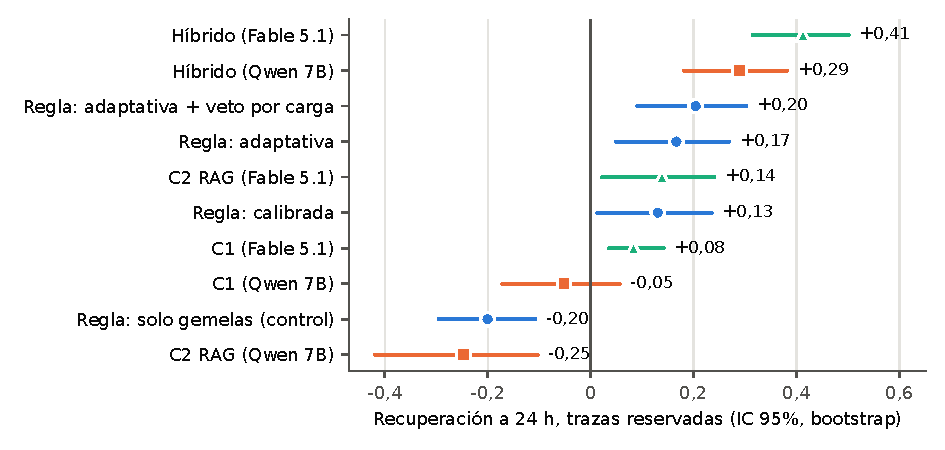
\includegraphics[width=\linewidth]{figures/es/fig_recovery.pdf}
\caption{Recuperación agregada en las trazas reservadas. Círculos: planificadores basados en reglas; cuadrados: Qwen2.5 7B; triángulos: Claude Fable 5.1.}
\label{fig:recovery}
\end{figure}

Con el modelo de 7B, los dos planificadores LLM que hacen ellos mismos el triaje de las alarmas quedan muy por debajo de las reglas. C1 se comporta como la heurística de solo gemelas (en la traza de desarrollo hizo el mismo número de reparaciones que el control de solo gemelas, con recuperaciones de $+0{,}80$ y $+0{,}78$ en un caso y de $-0{,}16$ y $-0{,}19$ en otro), y el conocimiento recuperado solo lo mejora modestamente. Limitar el LLM a vetar los candidatos de la regla adaptativa (híbrido) reduce aproximadamente un 40\,\% el coste de las falsas alarmas de la mejor regla, pero pierde detecciones.

Con el modelo de frontera, la clasificación cambia. El mismo diseño C2 alcanza $+0{,}58$, la recuperación agregada más alta de todos los planificadores. La figura~\ref{fig:tradeoff} sitúa cada planificador en el compromiso entre la recuperación ante fallos y el coste de actuar sobre el ruido.

\begin{figure}[t]
\centering
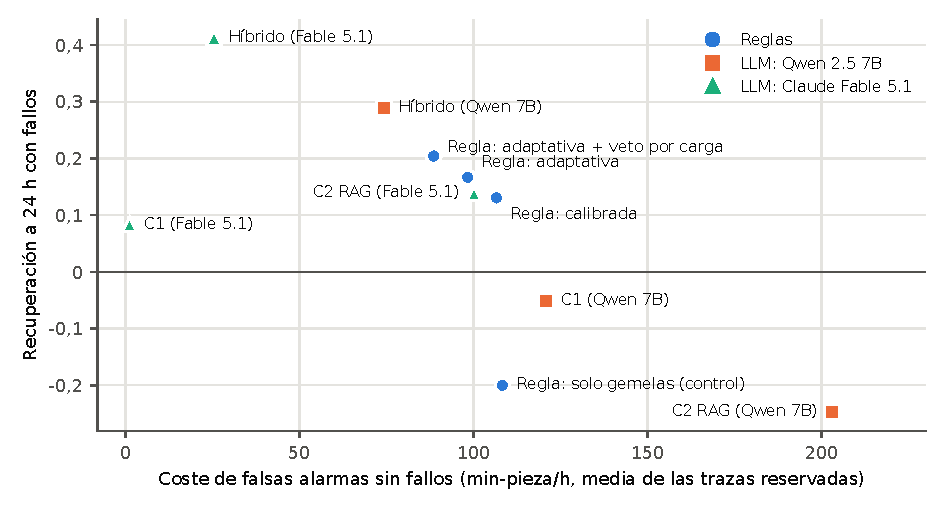
\includegraphics[width=\linewidth]{figures/es/fig_tradeoff.pdf}
\caption{Recuperación con fallos frente al coste de las falsas alarmas sin fallos, trazas reservadas.}
\label{fig:tradeoff}
\end{figure}

\subsection{Comparación estadística}
La tabla~\ref{tab:stats} compara C2 sobre Fable~5.1 con los demás planificadores. Pierde menos tiempo de producción que la mejor regla en 50 de 72 escenarios ($p=0{,}003$, ajustado por Holm), pero la diferencia de recuperación agregada, $+0{,}04$, tiene un intervalo de confianza que incluye el cero: gana a menudo y por poco, y en ocasiones pierde por más. El desglose por forma de fallo localiza la ventaja (figura~\ref{fig:shapes}): en los fallos en escalón y deriva los dos planificadores son indistinguibles; en los fallos intermitentes C2 sobre Fable~5.1 es mejor en 21 de 24 escenarios ($p=0{,}005$, ajustado por Holm). Los dos planificadores sobre Fable~5.1 son los únicos con recuperación agregada positiva en los fallos intermitentes. En los escenarios en que ambos actúan sobre la estación averiada, no hay evidencia de que actúe antes (diferencia mediana de 0~min, $p=0{,}17$).

\begin{table}[t]
\centering
\caption{C2 (RAG) sobre Claude Fable 5.1 frente a otros planificadores, pareado sobre los escenarios con fallo de las trazas reservadas. Valores $p$ de Wilcoxon ajustados por Holm dentro de cada bloque. $\Delta$: diferencia de recuperación agregada (positiva a favor de C2 sobre Fable 5.1), intervalo bootstrap estratificado al 95\,\%.}
\label{tab:stats}
\small
\resizebox{\linewidth}{!}{%
\begin{tabular}{lrrr}
\toprule
Frente a & Mejor en & $p$ (Holm) & $\Delta$ recuperación [IC 95\,\%] \\
\midrule
Adaptativa + veto por carga & 50/72 & 0{,}003 & $+0{,}04$ [$-0{,}01$; $+0{,}10$] \\
Regla adaptativa & 53/72 & $<0{,}001$ & $+0{,}06$ [$+0{,}01$; $+0{,}13$] \\
Regla calibrada & 63/72 & $<0{,}001$ & $+0{,}13$ [$+0{,}09$; $+0{,}18$] \\
C2 (RAG), Qwen 7B & 69/72 & $<0{,}001$ & $+0{,}38$ [$+0{,}31$; $+0{,}47$] \\
\midrule
\multicolumn{4}{l}{\emph{Frente a adaptativa + veto por carga, por forma de fallo}} \\
\quad escalón & 14/24 & 0{,}46 & $+0{,}01$ [$-0{,}06$; $+0{,}10$] \\
\quad intermitente & 21/24 & 0{,}005 & $+0{,}21$ [$\phantom{+}0{,}00$; $+0{,}42$] \\
\quad deriva & 15/24 & 0{,}46 & $+0{,}02$ [$-0{,}06$; $+0{,}10$] \\
\bottomrule
\end{tabular}}
\end{table}

\begin{figure}[t]
\centering
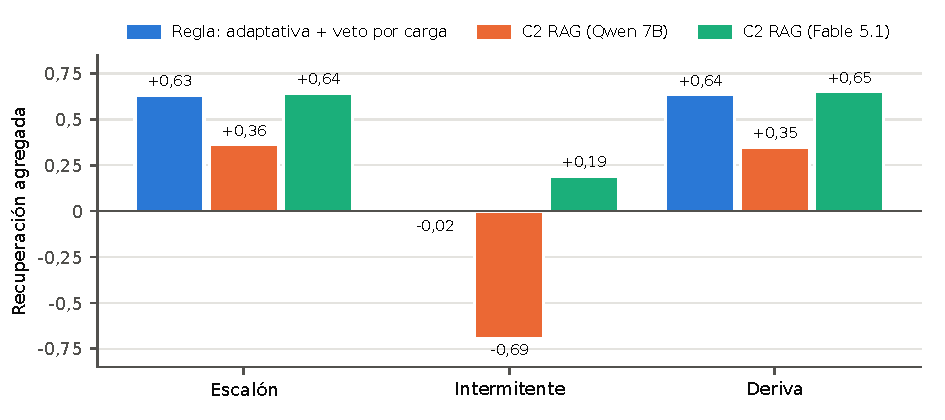
\includegraphics[width=\linewidth]{figures/es/fig_shapes.pdf}
\caption{Recuperación agregada por forma de fallo en las trazas reservadas.}
\label{fig:shapes}
\end{figure}

\subsection{El híbrido y el artefacto de las alarmas agrupadas}
El híbrido se comporta al revés con el modelo de frontera: se vuelve extremadamente conservador (5{,}1 reparaciones falsas por escenario, coste de falsas alarmas de 7 min-pieza/h) y pasa por alto la mitad de los fallos. Las razones que da lo explican. Fable~5.1 vetó al menos una estación en 1\,256 de sus 1\,437 llamadas, y el 98\,\% de esos vetos argumenta que las alarmas llegan en ráfagas compartidas por muchas estaciones y, por tanto, apuntan a una causa común de toda la línea; los 167 vetos de una estación que realmente estaba averiada dan todos esa razón. Por ejemplo, con L0\_S4 averiada: \emph{``Every alarm is a line-wide burst (all L0 stations plus L3) with twins alarming together; points to a common upstream cause, not individual faults. Hold off.''} (``Cada alarma es una ráfaga de toda la línea (todas las estaciones L0 más L3), con las gemelas alarmando juntas; apunta a una causa común aguas arriba, no a fallos individuales. Esperar.'') La inferencia es correcta; su premisa es un artefacto. El detector original emite una alarma \emph{solo} cuando más del 10\,\% de las estaciones se marcan en el mismo lote, de modo que toda alarma que produce es, por construcción, una ráfaga compartida. Con el modelo de 7B, el 17\,\% de los vetos da esta razón.

% =====================================================================
\section{Discusión}
\label{sec:discussion}

\paragraph{El cuello de botella es el triaje, no la planificación}
Una vez que una estación se juzga correctamente como averiada, basta una regla sencilla (desviar a una gemela libre, reparar). Todas las diferencias que medimos entre planificadores provienen de decidir qué alarmas merecen una acción. Cerrar el bucle del sistema de 2020 sin abordar esto habría empeorado la línea.

\paragraph{La capacidad importa donde el LLM hace el triaje}
El mismo diseño con recuperación aumentada pasa de $+0{,}20$ a $+0{,}58$ al sustituir el modelo de 7B por un modelo de frontera. Su ventaja sobre un test clásico de detección de cambios se concentra en los fallos intermitentes, cuyo patrón de encendido y apagado diluye las tasas de alarma pero deja un historial reconocible de alarmas y reparaciones. En los fallos en escalón y deriva, un test estadístico bien diseñado es igual de bueno, más barato y totalmente reproducible.

\paragraph{Un modelo capaz no puede reparar una interfaz Analyze--Knowledge deficiente}
Como veto sobre el detector heredado, el modelo de frontera fue menos útil que el de 7B, porque razonó correctamente sobre una evidencia cuya estructura producía el propio detector. En términos de MAPE-K, la información que pasa de Analyze a Plan (alarmas agrupadas) descarta precisamente la evidencia por estación que necesita el planificador. La implicación directa para la arquitectura es rediseñar esa interfaz, pasando evidencia por estación en lugar de alarmas agrupadas, antes de invertir en planificadores más capaces.

\paragraph{Los conjuntos de desarrollo engañan}
En la traza de desarrollo, tres conclusiones fueron erróneas: el planificador de 7B con recuperación aumentada parecía superar a la regla calibrada, el híbrido parecía dominar a su control y el modelo de frontera parecía equivalente al de 7B. Solo las trazas reservadas las invirtieron. Una sola traza con cuatro casos es demasiado pequeña para seleccionar diseños, y los controladores basados en LLM deberían evaluarse con datos que no se usaron para escribir sus prompts.

\paragraph{Amenazas a la validez}
\emph{De constructo}: los fallos son sintéticos y el modelo de efectos es aditivo y guiado por la traza, sin colas; sus parámetros no verificables se barrieron, y las conclusiones sobre el triaje se mantienen en todo el rango barrido, pero las recuperaciones absolutas dependen de ellos. La recuperación se mide solo en tiempo de producción, sin ponderación económica. \emph{Interna}: la métrica de acierto específico depende de una ventana de $\pm$120~min; el modelo de frontera no es reproducible bit a bit, aunque todas sus respuestas están almacenadas. \emph{Externa}: una sola línea de producción, un solo conjunto de datos y un solo detector heredado; dos modelos de lenguaje en los extremos de capacidad, sin tamaños intermedios. \emph{Estadística}: los escenarios de una misma traza no son independientes; remuestreamos dentro de cada traza, pero tres trazas reservadas siguen siendo un número pequeño de grupos.

% =====================================================================
\section{Conclusión}
\label{sec:conclusion}

Cerramos el bucle autonómico de una arquitectura de fabricación autocoordinada que, tal como se publicó, solo detectaba. Hacerlo de forma ingenua es perjudicial, porque el problema decisivo es el triaje de alarmas. Un test clásico de detección adaptativa de cambios es un baseline sólido. Un LLM de frontera con conocimiento operativo recuperado lo iguala en conjunto y lo supera claramente en los fallos intermitentes, mientras que el mismo diseño sobre un modelo de 7B no lo consigue. Usado como veto sobre alarmas agrupadas, el modelo de frontera es engañado por la propia estructura del detector. El trabajo futuro rediseñará la interfaz Analyze--Knowledge para pasar evidencia por estación, añadirá tamaños de modelo intermedios y validará el modelo de efectos con datos de planta con capacidades y tiempos de reparación reales.

% =====================================================================
\section*{Disponibilidad de datos y código}
\label{sec:availability}
El simulador sin interfaz gráfica, los planificadores, los prompts, el registro de desarrollo, las respuestas almacenadas de los modelos, los resultados y los scripts que producen cada tabla y figura están disponibles en \todo{URL del repositorio}. El conjunto de datos de Bosch es público~\cite{bosch2016kaggle}.

\section*{Declaración de contribución de autoría (CRediT)}
\textbf{Manuel S\'anchez:} conceptualización, metodología, investigación, visualización, redacción -- borrador original. \textbf{Ernesto Exposito:} supervisión, redacción -- revisión y edición.

\section*{Declaración de conflicto de intereses}
Los autores declaran no tener intereses financieros en conflicto ni relaciones personales conocidas que pudieran haber influido en el trabajo presentado en este artículo.

\section*{Declaración sobre el uso de IA generativa y tecnologías asistidas por IA en la preparación del manuscrito}
Durante la preparación de este trabajo los autores usaron Claude (Anthropic) para asistir en el desarrollo del software de simulación y análisis, redactar y revisar el texto del manuscrito, y como agente adversario que actuó como revisor para identificar debilidades y sugerir mejoras. El software fue revisado por el primer autor. Tras usar esta herramienta, los autores revisaron y editaron el contenido según fue necesario y asumen toda la responsabilidad sobre el contenido del artículo publicado. El uso de Qwen2.5 y Claude Fable~5.1 como planificadores forma parte del método estudiado en este artículo (sección~\ref{sec:planners}) y no guarda relación con la preparación del manuscrito.

\bibliographystyle{elsarticle-num}
\bibliography{refs}

\end{document}
